\documentclass[11pt,a4paper]{article}
\setlength{\parindent}{0 pt}
\usepackage[utf8]{inputenc}
\usepackage[spanish]{babel}
\usepackage{amsmath}
\usepackage{amsfonts}
\usepackage{amssymb}
\usepackage{makeidx}
\usepackage{graphicx}
\usepackage{lmodern}
\usepackage{kpfonts}
\usepackage{color}
\usepackage{epsfig}
\usepackage{multirow}
\usepackage{colortbl}
\usepackage[table]{xcolor}
\usepackage[left=2cm,right=2cm,top=2cm,bottom=2cm]{geometry}
\usepackage[utf8]{inputenc}
\usepackage{enumerate}
\usepackage[hidelinks]{hyperref}
\author{Miguel Angel Xamie Diaz Fuentes}
\begin{document}
\begin{center}
\begin{LARGE}
\textbf{PROYECTO G.A.A}
\end{LARGE}
\\
GRANJERO AUTÓNOMO AUTOSUSTENTABLE\\

\begin{figure}[hbtp]
\centering

\includegraphics[scale=0.30]{LOGO.png}
\end{figure}
Sistemas Eletrónicos De Interfaz\\
\begin{figure}[hbtp]
\centering

\includegraphics[scale=0.50]{UPZMG_Mecatr_nica.png}
\end{figure} 


Integrantes
\\\textit{
Cervantes Martínez Luis Osvaldo\\ 
Diaz Fuentes Miguel Angel Xamie \\
Hernandez Sanchez Rafael\\
Jiménez Cortéz Raúl\\
Reyes Alvarez Ulises Isaac
}
\\Maestro
\\\textit{Morán Garabito Carlos Enriquez}
\end{center}

\footnote{Universidad Politécnica De La Zona Metropolitana De Guadalajara} 

\pagebreak

\section{Planteamiento del problema}
\subsection{¿Cuál es el problema a resolver?}
Evitar costos elevados, daños y emisiones contaminantes.\\
\subsection{¿Porque se desea resolver esta problemática?}
Reducir presupuesto para la reinversion, mano de obra, producción, material y maquinaria. Evitar que el capital humano sea afectado por lesiones en la piel por radiaciones solares (desidratación, cáncer, arrugas, rozaduras, reacciones alérgicas). Evita el calentamiento global, reduce el uso de combustibles fósiles y contribuye a un desarrollo sostenible.
\section{Desarrollo} 
\subsection{Reunir}
Existen personas que porque la economía se meten a trabajar en el campo, ya que trabajar en ello genera dinero suficiente para alimentar a una familia, pero algunas personas ya no quieren trabajar en ello ya que es un trabajo muy pesado y prefieren buscar en otro lado porque no cuentan con seguro medico o el dinero suficiente para tratar alguna enfermedad de ellos mismos causados por los rayos solares.\\
Causa de esta los ingenieros agrónomos se están quedando sin trabajadores, lo que está ocasionando que los ingenieros tengan que trabajar o poner a sus hijos a hacer el trabajo, quitándole el tiempo.
\subsection{Determinar}
La importancia en este proyecto es cuidar la salud de los trabajadores, ya que algunos no cuentan con sus recursos necesarios para los gastos médicos, ya que este proyecto aumentara el capital de ingresos a los dueños de sus hectáreas agrícolas.
\subsection{Identificar}
El ingeniero agrónomo se está viendo afectado por la falta de trabajadores, la economía en costos de transportación y uso de maquinaria pesada.
\subsection{Proponer}
En este año hemos sentido que la temperatura del planeta está aumentando, lo que esta afectando a los trabajadores del campo ya que están trabajando bajo las consecuencias de los rayos ultravioletas generándoles problemas graves a su salud, causa de esto ya las personas no quieren trabajar en el campo.\\
El uso de maquinaria genera usar combustibles fósiles tanto para la transportación de ellos mismos como el uso para el sembradío generando gases contaminantes para el medio ambiente, lo que genera contaminación al medio ambiente y el calentamiento global.
\subsection{Encontrar}
La solución para esto es poder diseñar un proyecto para sustituir a los trabajadores, para que no existan las lesiones hacia los trabajadores por causa de la radiación solar y teniendo solo una persona operando nuestro equipo. La transportación sería más rápida y reduciendo los gases contaminantes de la maquinaria pesada, así como reducir gastos por trabajadores, combustible y transportación.

\footnote{Universidad Politécnica De La Zona Metropolitana De Guadalajara} 
\pagebreak

\subsection{Hallar}
Ayudar al ingeniero agrónomo a no exhibir a sus trabajadores a altas radiaciones ultravioletas que puedan ocasionarles daños severos, reducir gastos y ayudar a reducir contaminantes hacia el medio ambiente.
\subsection{Analizar}
Queremos brindarle a los ingenieros agrónomos apoyo en sus tierras con ayuda de tecnología. con un fácil manejo al sistema, reduciendo gastos, contaminación al medio ambiente y tiempo. También promover la tecnología con energía renovable y con puntos que favorezcan a no contaminar en muchos aspectos.
\section{Planteamientos}

\begin{itemize}

\item ¿Tendrá nuestro proyecto beneficios a largo plazo?\\
\item ¿Generará o perderá empleos?\\
\item ¿Tendrá un beneficio hacia los ingenieros agrónomos?\\
\item ¿Lograŕa sustituir fácilmente a la maquinaria pesada o capital humano?\\
\item ¿Será realmente amigable con el medio ambiente?\\
\end{itemize} 

\section{¿A dónde queremos ir?}

Lograr una autosustentabilidad un poco mas alta en el capital del ingeniero agrónomo ya que también cuida el medio ambiente en no usar maquinaria pesada utilizando el medio de combustible diesel, ya que con este proyecto ayuda al medio ambiente por el motivo que utiliza la energía solar y también ayudara a los trabajadores a que no tengan alguna enfermedad que se pueda producir en las horas de trabajo con el peso del tiempo, he así este podrá tener un conteo mutuo por hectárea de cuántas semillas se sembraron y ayudar al dueño del terreno a realizar trabajos sin tener que cansarse o asolearse, debido que seria por personal autorizado.\\\\
\textbf{Usando la tabla en la parte inferior explica cuáles objetivos son desarrollados en las materias que se están cursando y en las que se cursaran en los dos siguientes cuatrimestres.}\\
Vamos a generalizar la explicación dando el uso de cada verbo con respecto al los objetivos planteados y que se desarrollan en las materias cursadas y las posteriores a cursar.\\\\
\textit{° \textbf{Determinar} la misión y visión del proyecto de acuerdo a los avanzes del mismo.\\
° \textbf{Verificar} que el proyecto sea viable y el desarrollo del mismo cumpla con los puntos que estamos mencionando y esto con ayuda de la evaluación que se realiza al proyecto por parte de la academia.\\
° \textbf{Definir} que realizará el proyecto y de qué manera lo hará con respecto a los cliente ¿s y a la hora de una demostración, con ayuda de ética y presentaciones en inglés.\\
° \textbf{Identificar} el problema que queremos atacar o innovara el proyecto en esa área.\\
° \textbf{Diseñar} un proyectó con respecto a los puntos que mencionamos y cumpla parámetros de diseño para la venta y seguridad del producto (garantía).\\
° \textbf{Conocer} el área de mercado en la que compite el proyecto y a su vez la competencia.\\
° \textbf{Evaluar} los respectivos documentos para la presentación del producto en todos sus puntos.\\
° \textbf{Estudiar} los temas que involucran las funciones del proyecto interior y exterior.\\
° \textbf{Describir} como el proyectó utiliza cada parte de las materias si esta aporta algo.\\
° \textbf{Proponer} mejoras de cada parte del prototipo a su vez como el la visión o misión del proyecto.\\
° \textbf{Plantear} problemas más problemas para ir mejorando constantemente.\\
° \textbf{Formular} situaciones en las que el proyecto tendría que actuar, cambiar o mejorar para atacarlas y sean aprovechables.\\
° \textbf{Analizar} todo el desarrollo del proyecto, realizando bitácoras o un registro de todo lo sucedido para cualquier situación.\\
° \textbf{Corroborar} todo antes de cada prueba.\\ }



\begin{table}
\centering
\begin{tabular}{lllll}
Determinar & Verificar & Definir & Identificar \\ \hline 
Diseñar & Conocer & Evaluar & Elaborar \\ \hline
Estudiar & Describir & Proponer & Plantear \\ \hline
Formular & Analizar & Corroborar &  \\ \hline
\end{tabular}
\end{table}


\section{Objetivos}

Para desarrollar este proyecto con éxito teniendo una visión y misión de acuerdo al planteamiento del problema es necesario que sea viable con un buen esquema del mismo, marcando los puntos importantes (causas,motivos,beneficios,etc). Realizando las fases de desarrollo aplicándolas constantemente y aprendiendo de los resultados, crear a su vez la idea a los agrónomos para que estos mismos tengan interés en estos productos es 
una parte esencial porque sin demanda no hay venta alguna. Por otra parte las ventajas deben ser considerables y de fácil acceso al consumidor.
Todo se desarrollará con un buen trabajo en equipo, un esquema completo de todas las categorías del proyecto para una solución adecuada en caso de un problema, verificar la viabilidad del proyecto, identificar la competencia en el mercado y el área en que estaremos, tener un organigrama y diagramas de ganck.
\footnote{Universidad Politécnica De La Zona Metropolitana De Guadalajara} 
\section{Justificación}
 Para el desarrollo de este proyecto nos motivó la idea de dar un crecimiento exponencial a la agricultura con el uso de la tecnología con suministro de energía renovable, trabajando de forma autónoma, reduciendo el tiempo, el no uso de combustible fósil, velocidad de trabajo, limpieza y desarrollo sostenible en esta área. Esta idea también tiene una visión que no es muy costosa y el mantenimiento es muy bajo en costos y fácil de llevar a cabo. Trabajaría principalmente en la siembra de tierra con un cronograma basado en lo que el agricultor necesita, para futuros desarrollos del mismo se tiene en mente programas para desarrollar estos robots de manera renovable, ya sea en plásticos o en metal reciclado.
 
 \section{Delimitación}
 El proyecto tiene como visión ser un proyectó rentable en el área de la agricultura con un uso que favorezca los puntos mencionados anteriormente como son (medio ambiente, gastos, uso). Ofrecer un servicio que satisfaga al cliente y cumpla las necesidades solicitadas en base a la función del proyecto cumpliendo también con calidad, resultados y ganar un prestigio para ir mejorando nuestros productos en cuanto a funciones y áreas de trabajo. Como visión estar a un nivel más alto que nuestros competidores y ser un empresa que marque diferencias en el uso de tecnología renovable y autónoma.
 
 \pagebreak
 \section{Matriz De Roles}
 
 \begin{itemize}
 \item - Reyes Álvarez Ulises Isaac (\textbf{Ensamblador})\\
 \item - Cervantes Martínez Luis Osvaldo (\textbf{Programador})\\
 \item - Jiménez Cortes Raul (\textbf{Diseñador})\\
 \item - Hernández Sánchez Rafael (\textbf{Secretario})\\
 \item - Diaz Fuentes Miguel Angel Xamie (\textbf{Desarrollador})\\ 
 \end{itemize}
 
 \section{Diagrama GANTT}
 \begin{figure}[hbtp]
 \centering
  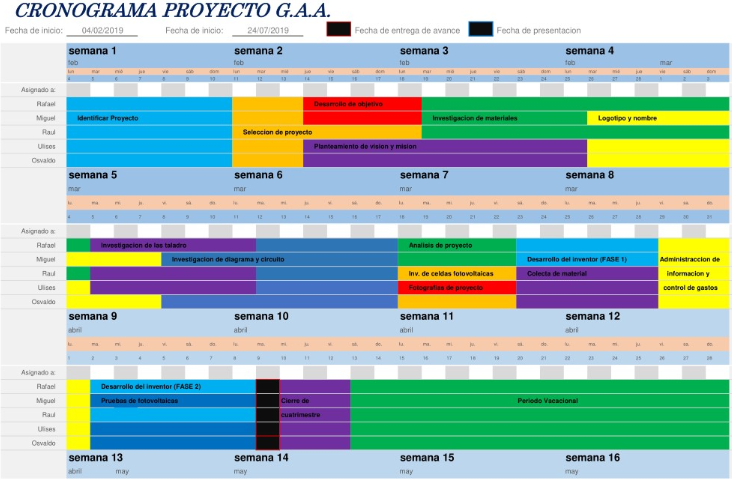
\includegraphics[scale=0.85]{Diagrama(01).png} 
 \end{figure}
  \footnote{Universidad Politécnica De La Zona Metropolitana De Guadalajara} 
  \pagebreak
 \begin{figure}[hbtp]
 \centering
  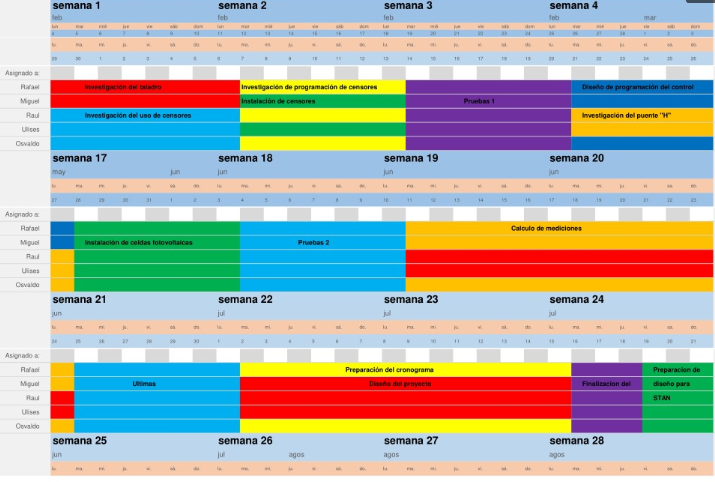
\includegraphics[scale=0.85]{Digrama(02).png} 
 \end{figure}
\begin{figure}[hbtp]
 \centering
  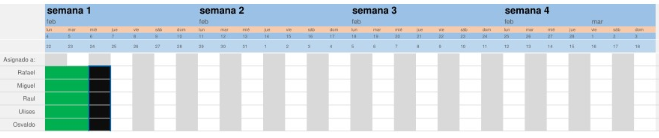
\includegraphics[scale=0.85]{Diagrama(03).png} 
 \end{figure}
  \footnote{Universidad Politécnica De La Zona Metropolitana De Guadalajara} 
\pagebreak

\section{Matriz De Costos y Materiales}
\begin{table}[htb]
\rowcolors{2}{blue!15}{white}
\centering
\begin{tabular}{|p{7cm}| p{1.5cm}|}
\hline
  \rowcolor{blue!50}              % Heading with different color to highlight it     
\multicolumn{2}{|c|}{\textbf{PRESUPUESTO}} \\
\hline \hline
Batería Lipo & \textdollar1200 \\ \hline 
Paneles Solares & \textdollar500 \\ \hline
Arduino Mega & \textdollar360 \\ \hline
Piezas Metálicas & \textdollar800 \\ \hline
Moto Reductores & \textdollar60 \\ \hline
Cables Dupon & \textdollar80 \\ \hline
Power Bank & \textdollar300 \\ \hline
Cinta Doble Cara & \textdollar35 \\ \hline
Cilicon y Colaloca & \textdollar30 \\ \hline
Dos Llantas & \textdollar40 \\ \hline
Leds & \textdollar10 \\ \hline
Baquelita & \textdollar18 \\ \hline
Tranistores & \textdollar8 \\ \hline
Resistencias & \textdollar30 \\ \hline
Capacitores & \textdollar6 \\ \hline
Servomotor & \textdollar60 \\ \hline
Ultrasonido & \textdollar80 \\ \hline
Bluethoot Arduino & \textdollar75 \\ \hline
Madera Triplay & \textdollar125 \\ \hline
Cable de Impresora  & \textdollar60 \\ \hline
Apagadores Switch & \textdollar15 \\ \hline
Palitos de madera & \textdollar30 \\ \hline
TOTAL & \textdollar3922 \\ \hline
\end{tabular}
\caption{Cotización de Materiales.}
\label{tabla:anchofijo}
\end{table}
\footnote{Universidad Politécnica De La Zona Metropolitana De Guadalajara} 
\pagebreak

\section{Aportación de cada materia cursada en el cuatrimestre al proyecto}
\textbf{INGLÉS IV:}\\ Desarrollo de presentaciones y exposiciones con el uso de este idioma para una demostración de calidad y competencia con otros proyectos.\\\\
\textbf{ÉTICA PROFESIONAL:}\\ La formalidad que debe llevar el reporte y presentaciones del proyecto así como su estructura, también verificando que nuestro proyectó no pueda llegar ser copiado por otra persona.\\\\
\textbf{ESTRUCTURA Y PROPIEDADES DE LOS MATERIALES:}\\ Uso adecuado de la estructura del proyecto y delimitar su resistencia, calidad, vida útil del producto y seguridad para demostrar sus especificaciones de venta.\\\\
\textbf{PROGRAMACIÓN DE PERIFÉRICOS:}\\ El uso de lenguajes como C y Python entre otros para la programación del prototipo y funciones mecánicas.\\\\
\textbf{SISTEMA ELECTRÓNICOS DE INTERFAZ:}\\ Uso de puertos(circuito físico) para la transmisión de señales o recepción de las mismas desde sistemas o subsistemas hacia otro. Y con esto establecer especificaciones técnicas concretas.\\\\
\textbf{CONTROLADORES LÓGICOS PROGRAMABLES:}\\ Para el uso de procesos productivos industriales para el ahorro de costes y tiempo, con la finalidad de reducir el mantenimiento y alargar la vida útil.
\pagebreak
\section{Desarrollo}
La primera etapa se realizó en la parte superior en la cual podemos encontrar los paneles solares que se conectaran con el centro de carga del proceso y también poder alimentar algunos sectores de iluminación.
Elegimos también hacerlo de forma inclinada por si se presentaran lluvias este no genere acumulaciones en su parte superior.
En la etapa 2 se realizaron las conexiones de las salidas de los paneles y al mismo tiempo por trabajo dividido se empezó a conectar los motores a la base principal y su puente H para el control de dirección. En la parte trasera se asigna el lugar de sistema central control por espacio y un buen orden de conexiones.
También desarrollamos el circuito de intermitentes de la parte frontal, primero se creó en Proteus, se realizó el PCB y se procedió a imprimirlo y realizar el proceso de baquelita al pegar el circuito en modo espejo por medio de una plancha y luego sumergirlo en cloruro férrico.\\\\
Se llevo acabo una baquelita que iría en la parte frontal del granjero, esto para demostrar también que un proyecto puede generarse de muchas maneras ya sea con circuitos o sensores ya preestablecidos para solo programarlos o crear todo el circuito desde cero.\\\\
El circuito que esta en la parte frontal funciono perfectamente este nos permitirá alumbrar de noche o también se puede asignar para alarmar en caso de a ver entrado en colisión y este atascado o dañado.
Luego una vez terminado esto la etapa 3 fue crear la base que sostendrá los paneles y también ubicar los cables de conexión con los motores, servomotores, ultrasonido y control bluethoot. Esto es lo más importante ya que al no asignar bien los espacios y conexiones retrasa mucho por el techo de carga el cual tapa toda la parte central de control el cual se pega una vez terminado todo.\\\\
La última etapa 4 y la más importante fue crear el control del granjero en APP Inventor, realizar las pruebas necesarias, desarrollar el código del robot, también configurar el sensor ultrasonido para la visualización sonar, en esta etapa del sonar verificamos un problema el cual era que no podía funcionar al mismo tiempo que mandábamos señal con la aplicación ya que al transmitir datos al bluethoot el ultrasonido también necesitaba eso y creaba interferencias así que los explicábamos individuales.\\\\
Por la parte delantera esta el que sería el almacenaje y control de semillas por distancia recorrida en el observamos que elegimos un comportamiento inclinado para no tener que realizar una función de caída de la semilla y solo sea por gravedad y una compuerta de control.
Por último, el ajuste de tornillos, cintas, control, aspecto, cables, y piezas de movimiento. El proyecto fue muy interesante desarrollarlo ya que se tuvo que realizar una investigación de todos los componentes que lo conforman y que se tiene que realizar para la evolución del mismo con el tiempo esperemos poder hacer este objetivo realidad conforme el desarrollo del mismo en futuras prácticas.
\begin{figure}[hbtp]
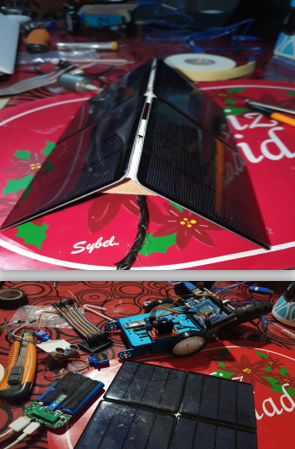
\includegraphics[scale=0.50]{02.png}
\end{figure} 
\begin{figure}[hbtp]
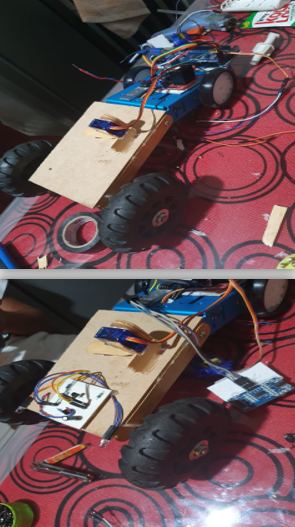
\includegraphics[scale=0.50]{03.png}
\end{figure} 
\begin{center}
\pagebreak
PRESENTACIÓN FINAL
\end{center}
\begin{figure}[hbtp]
\centering
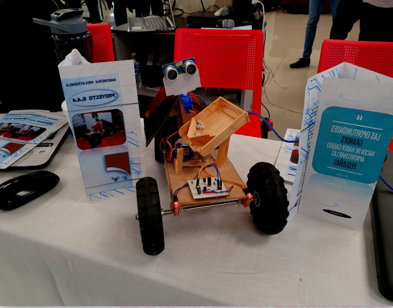
\includegraphics[scale=0.50]{portada.png}
\end{figure} 
\pagebreak

\begin{thebibliography}
 \\Referencias URL...
\end{thebibliography}
\url {https://www.iluminet.com/funcionamiento-paneles-fotovoltaicos-energia-solar/}\\
\url{https://dmsolar.mx/celdas-fotovoltaicas-tipos-y-su-funcionamiento/}\\
\url{http://electronicayciencia.blogspot.com/2010/09/receptor-coche-rc-de-dos-canales.html}
\\
\url{http://panamahitek.com/el-puente-h-invirtiendo-el-sentido-de-giro-de-un-motor-con-arduino/}\\
\url{https://greenercorp.com/wp-content/uploads/wp_disenos_de_filos_para_cuchillas.pdf}






\end{document}